\subsection{Rejecting out-of-distribution input}
\label{sec:ood}

We asked whether the confidence signal of Section~\ref{sec:abstention} also identifies
input the network was never trained on, holding an MNIST-trained model fixed while
presenting KMNIST, notMNIST, Fashion-MNIST, and SVHN, with $\tau$ calibrated on held-out
MNIST alone. At $\alpha = 0.025$, a threshold refusing $2.6\%$ of MNIST, it refuses only
$12.7$–$26.8\%$ of out-of-distribution input, and two detectors that exclude the network
outperform it: mean image intensity reaches $\mathrm{AUROC}$ $0.980$ and the residual
outside MNIST's top-$50$ principal subspace $0.971$–$0.999$, against $0.694$–$0.870$ for
the network (Figure~\ref{fig:ood}). KMNIST is the exception: it is the only probe whose
evoked firing rate matches MNIST's ($0.00213$ against $0.00225$), and there the intensity
baseline falls to $0.745$ while the network attains $0.870$ — its confidence carries
novelty information that brightness does not, precisely where brightness fails. Both
observations rest on a single trained network.

\begin{figure}[t]
\centering
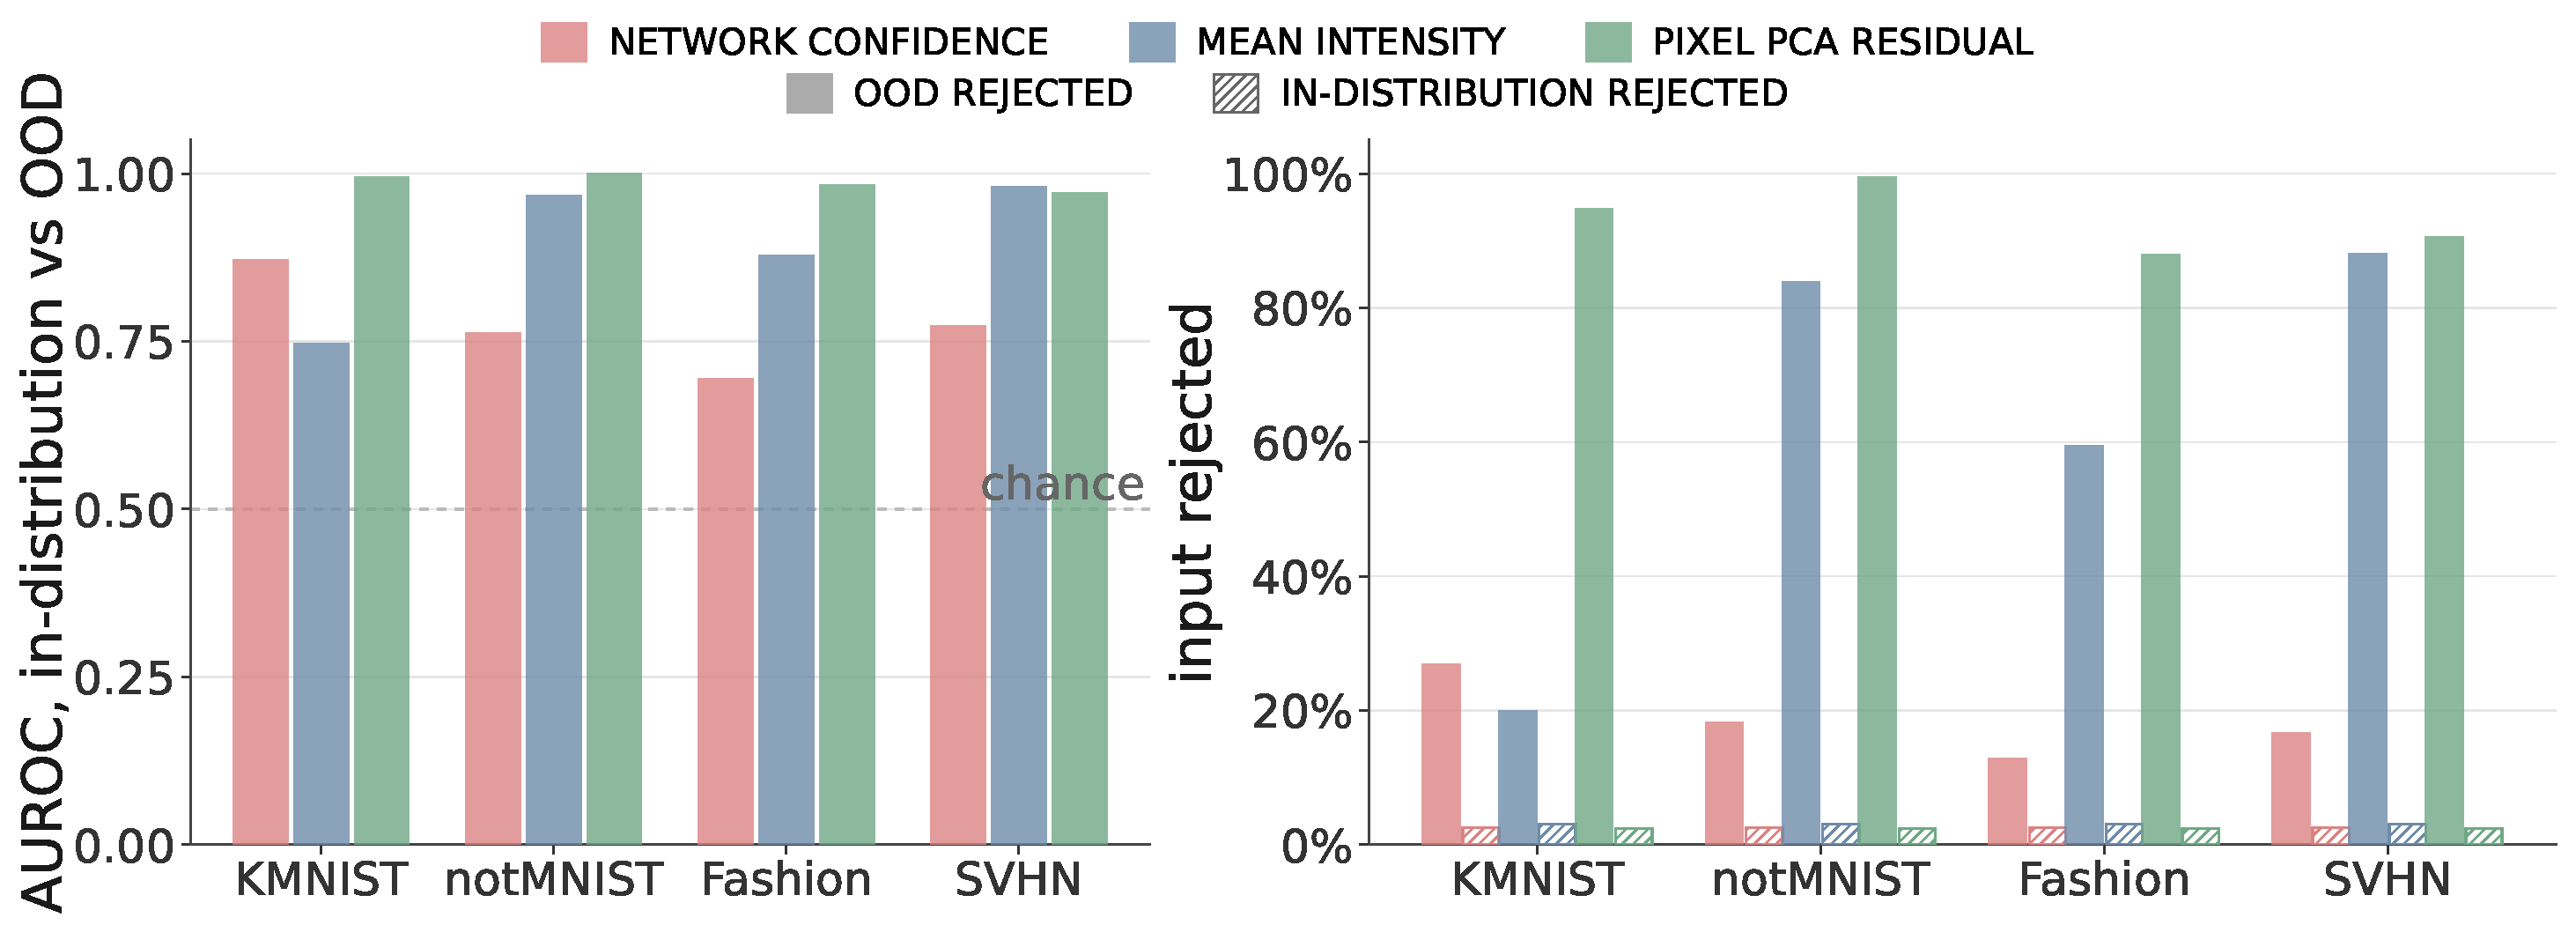
\includegraphics[width=\textwidth]{figures/ood_rejection.pdf}
\caption{Out-of-distribution rejection by an MNIST-trained supervised model.
\textbf{Left:} separability between MNIST test input and each out-of-distribution set, as
$\mathrm{AUROC}$ of the network's predictive entropy against two detectors computed on raw
pixels that use no network at all. \textbf{Right:} the fraction of out-of-distribution
input refused at a threshold calibrated on held-out MNIST at $\alpha = 0.025$; the dashed
line marks the $2.6\%$ of in-distribution input the same threshold refuses. Probes are
ordered by decreasing similarity of low-level image statistics to MNIST.}
\label{fig:ood}
\end{figure}
